%!TEX root = ../VorlageBA.tex
\chapter{Grundlagen aus dem IoT für das Thema Smart Home Interior}
\label{cha:grdl}

\addtocontents{toc}{\protect\setcounter{tocdepth}{1}}
\section{Smart Home Aufbau und Funktion}
Ein Smart Home ist ein System, welches automatisch smarte Geräte im Haus steuert. Die smarten Geräte können zusätzlich durch den Nutzer im Haus gesteuert werden. Ein smartes Gerät ist smart, wenn es mit einem Computer ausgestattet ist und damit die Funktionalität des Gerätes erweitert. Dies ist durch verschiedene Kommunikationsmethoden möglich. Diese Kommunikation kann z.B. durch Bluetooth, WiFi oder auch Infrarot durch den Nutzer und der Smart Home Automatisierung eintreten. Für den Prototypen der Bachelorarbeit wird ein Wireless System verwendet. Dies bedeutet, dass kein Kabel für die Kommunikation nötig ist. Die Verwaltung der Kommunikation der sendenden und empfangenden Geräte führt das MQTT-Protokoll durch. Kapitel \ref{sec:mqtt} erläutert den Aufbau und die Funktionen von MQTT. 
\newline
Weiterhin ist es möglich durch die Automatisierung bestimmte Interaktionen im Haus nicht mehr manuell vom Bewohner im Haus ausführen zu müssen. Für jeden Raum wird in der Regel eine unterschiedliche Automatisierung erstellt, da zu unterschiedlichen Zeiten andere smarte Geräte im Raum benutzt werden. Dadurch sorgt das Smart Home für Einsparungen im Haus.
\newline
Ein Beispiel für eine Einsparung ist der Stromverbrauch. Dabei passiert es oft, dass Strom im Haus verbraucht wird. Dieser kommt von Geräten, die nicht durchgehend Strom brauchen. Ein Smart Home kann die smarten Geräte so verwalten, dass sie nur dann Strom verbrauchen, wenn sie auch wirklich vom Nutzer aktiv verwendet werden. Sollte der Nutzer ein Gerät nicht mehr brauchen, kann das Smart Home den Stromkreis automatisch unter festgelegten Bedingungen unterbrechen. Zusätzlich können damit gefährliche Situationen vermieden werden, wie z.B. ein Kurzschluss. \citep{sripan2012research}
\newline
Es ist auch wichtig hervorzuheben, dass an Smart Homes bestimmte Anforderungen gestellt sind, damit Kriterien wie Sicherheit, Komfort oder Mobilität bei Älteren und Menschen mit Behinderung gewährt sind. Diese Anforderungen für die genannten Personen werden in \citep{das2015design} dargestellt und ein Prototyp veranschaulicht eine mögliche Lösung, um diese Anforderungen zu erfüllen. Aus diesen Erkenntnissen ist es möglich, verschiedene Smart Home Systeme zu entwickeln. Diese können speziell an die Nutzer angepasst werden. So haben Personen, die ohne Hilfe ihren Alltag nicht mehr bewältigen können oder Personen, die medizinische Unterstützung brauchen, die Möglichkeit, trotzdem selbstständig zu leben. Außerdem bringt die Erweiterung zu einem Smart Home den positiven Aspekt der Zeiteinsparung mit sich. Durch die verschiedenen positiven Gründe steigt auch die Relevanz der Smart Homes immer weiter an. Besonders die Einbindung von Machine Learning Methoden hebt die Relevanz weiter an.

\section{Relevanz neuronaler Netze in Smart Homes}
Ein neuronales Netz ist in der Lage das Verhalten von Menschen zu erkennen, um so in Smart Homes unter anderem das Strom Management zu verbessern. Anhand von Sensoren wird gemessen, wie viele Personen sich im Raum befinden und was sie wirklich an Strom brauchen. Anhand der Sensorwerte und dem Verhalten der Menschen entscheidet das neuronale Netz, welches Gerät ausgeschaltet werden kann. \citep{badlani2011smart} Aus dieser wissenschaftlichen Arbeit mit dem genannten Beispiel zum Strom Management ist zu erkennen, dass ein neuronales Netz durch Interaktionen mit Sensoren in der Lage ist, die Steuerung der smarten Geräte zu verwalten. Deshalb ist es für den Autor wichtig, sich mit der Verbindung zwischen neuronalen Netzen und Smart Homes zu beschäftigen.
\newline
Weiterhin ist besonders beachtenswert, dass Smart Homes im Zusammenhang mit neuronalen Netzen auch beeinträchtigen Personen Unterstützung bieten. Diese sollen dadurch weiterhin selbstständig leben können, wie die fremde wissenschaftliche Arbeit \citep{hussein2014smart} darstellt. 
\newline
Anhand dieser wissenschaftlichen Arbeiten werden zudem weitere Beispiele gezeigt, wie man neuronale Netze in Smart Homes einsetzen kann. Der Autor will damit hervorheben, dass sich die Umsetzung des Prototypen  in ein Smart Home integrieren lässt. Die verschiedenen Systeme, die für ein Smart Home entwickelt werden und von einem neuronalen Netz verwaltet werden, nutzen oft mehrere unterschiedliche neuronale Netze. Daraus stellt sich die Frage, ob für ein Smart Home ein oder mehrere neuronale Netze von Vorteil sind. Dies lässt sich anhand der wissenschaftlichen Arbeiten, die in diesem Kapitel ausgeführt wurden und dem Prototypen der Bachelorarbeit beantworten. Deshalb ist es besser für verschiedene Räume unterschiedliche neuronale Netze zu nutzen, da diese unterschiedliche Steuerungen im Haus damit übernehmen und die Aufgaben, damit übersichtlicher bleiben. Dies zeigt, dass neuronale Netze in Smart Homes eine große Rolle übernehmen. So kann dadurch auch z.B. die Möglichkeit Möbel in einem Smart Home zu digitalisieren in Betracht gezogen werden.

\section{Smart Home Interior}
Mit diesem Kapitel erläutert der Autor eines der beiden Hauptgebiete in dieser Bachelorarbeit. Es wird hauptsächlich die Frage geklärt, welche Rolle Möbel in einem Smart Home spielen, wenn man diese zu smarten Geräten weiterentwickelt. Zusätzlich werden verschiedene Möglichkeiten gezeigt, wie dies umgesetzt werden kann.

\subsection{Die Funktion der Innenausstattung im Smart Home}
Das Teilgebiet Smart Home Interior zeigt die Digitalisierung der Innenausstattung in einem Smart Home. So wird veranschaulicht, dass die Möbel im Haus oder der Wohnung als smarte Innenausstattung genutzt werden können. Um smarte Umgebungen zu erschaffen, werden die bereits bestehenden Möbel zu smarten Geräten umgewandelt. Damit könne smarte Geräte die ein Smart Home definieren, bestimmte Aufgaben an Möbel abgeben oder ihnen weitere Informationen zur Automatisierung mitteilen. Dadurch entstehen weitere Steuerungen, die Smartphones oder andere Geräte ersetzen. 
\newline
Sitzmöbel werden z.B. als Steuerung anderer smarter Möbel oder Geräte eingesetzt. Der Sofaprototyp soll dies darstellen und zeigen, wie es die Aufgaben eines Smartphones oder ähnlichen Geräte ersetzt. Außerdem ist es möglich, für die Möbel eine zusätzliche Automatisierung zu entwickeln und in das Smart Home mit zu integrieren. Smarte Möbel dienen zur passiven Steuerung von smarten Geräten oder Möbelstücken ohne, dass der Nutzer bei der Interaktion selbst etwas davon äußerlich an der Innenausstattung mitbekommt. Der Nutzer muss nicht mehr aktiv ein Tablet oder ähnliches Gerät entsperren, die App raussuchen und darüber steuern, sondern braucht nur noch eine aktive Interaktion mit den Möbeln und steuert so die smarten Geräte. Dadurch hat er einen geringeren Einfluss auf die individuelle Steuerung der Geräte. So spart der Nutzer aber wiederum Zeit. Da die Steuerung durch die Interaktionen verwaltet werden muss, zeigt \citep{soares2010embedding} wie es möglich ist, dass ein Möbelstück mit einem neuronalen Netz verknüpft werden kann.

\section{Neuronale Netze zur Klassifizierung}
\label{sec:NNK}
Das folgende Kapitel befasst sich mit Grundlagen zu neuronalen Netzen. Umfasst wird dabei der Aufbau, wie die Berechnungen auf den Layern stattfinden, wie klassifiziert wird und Allgemeinbegriffe werden geklärt. Da das Thema zu neuronalen Netzen sehr breit ist, wird hier nur das erläutert, was der Autor zur Umsetzung und Evaluation in den späteren Kapiteln benutzt. So sollen später benutzte Fachbegriffe und Methoden nicht in jedem Kapitel neu erklärt werden.

\subsection{Aufbau eines neuronalen Netzes}
Das neuronale Netz ist in Schichten, auch Layer \(L\) genannt, aufgebaut. Es besteht aus einem Input-, Hidden- und Output-Layer. Die Zahl der Hidden-Layer ist immer \(L - 2\). Der Input-Layer bekommt die Daten der Außenwelt in Zahlenwerten beschrieben. Jeder einzelne Wert wird an eine Input-Unit im Layer übergeben. Daraufhin werden die Daten weiterverarbeitet und an die Hidden-Units in den Hidden-Layern gesendet. Es können mehrere Hidden-Layer je nach Aufgabe des neuronalen Netzes benutzt werden. Von dort aus werden diese Werte mit den Gewichtungen zusammen gerechnet und an eine Aktivierungsfunktion übergeben. Die nächsten Schritte werden in den folgenden Kapiteln weiter erläutert. Nach den Hidden-Layern kommt als letztes der Output-Layer mit den Output-Units. Der Output-Layer gibt die Zahlenwerte aus, die die Vorhersage des neuronalen Netzes als Ergebnisse in Form von Zahlenwerten liefern. Für diesen in der Bachelorarbeit verwendeten Prototypen ist im neuronalen Netz jeder Layer mit dem vorheriegen Layer verbunden. 

\subsection{Initialisierung der Layer und Inputwerte}
Zu Beginn, wie schon erwähnt, liest das neuronale Netz die Inpurtwerte in den Inputlayer ein. Zusätzlich sollte nach dem Input-Layer pro Layer auch noch der Bias-Wert als weitere Unit im Layer hinzugefügt werden, da sonst wie z.B. bei der Linearen-Aktivierungsfunktion der Achsenabschnitt nicht geändert wird und die Funktion damit nicht so stark verschoben werden kann, wie mit dem Bias-Wert. 
\newline
Benutzt man Bibliotheken wie Keras, müssen die Aktivierungsfunktion und der Bias-Wert als optionale Parameter im Layer angegeben werden. Außerdem muss beim Dataset angegeben werden, wie viel Prozent der Datensätze als Testdaten verwendet werden sollen. Diese Parameter sind vom Autor schon in der Initialisierung angegeben, da dies bei der Ausführung des neuronalen Netzes schon angegeben sein muss. 
\newline
Da für das Netz eigene Datensätze genutzt werden, werden diese noch normalisiert, um die Daten besser an das Netz anpassen zu können und das globale Minimum der Fehlerrate besser zu erreichen. 

\subsection{Feedforward und Backpropagation}
\label{sub:fee_back}
Der Feedforward und die Backpropagation sind die Hauptausführungen des neuronalen Netzes. Im Feedforward Schritt werden aus den Inputwerten die Vorhersagen getroffen. In der Backpropagation wird die Fehlerrate dieser Ergebnisse angepasst, sodass die Vorhersagen im Endergebnis so nah wie möglich an den Soll-Werten liegen.

\subsubsection{Berechnung der Inputwerte}
Zwischen den einzelnen Layern sind Gewichtungen  \(x_1 \dots x_n\), welche willkürlich zu Beginn gewählt werden. Diese werden mit den Eingabewerten  \(a_1 \dots a_n\) multipliziert und als Summe in der Funktion \(h\) ausgerechnet. Abbildung \ref{fig:h_nn} zeigt ein Perzeptron, welches die Verbindung zwischen den Input- und Output-Units einzeln darstellt. Ein Perzeptron ist das einfachste neuronale Netz mit nur einer Output-Unit. Die vorherigen Layer können jedoch mehr Units besitzen.
\newline
\[\displaystyle h(x)=\sum_{i=1}^{n} a_i x_i = (a_1 \cdot x_1 + a_2 \cdot x_2 + \dots + a_{n-1} \cdot x_{n-1} + a_n \cdot x_n)\]

\begin{itemize}
    \RaggedRight\item[] \(a_n\):  Inputwerte aus der Realwelt
    \RaggedRight\item[] \(x_n\):  Gewichte
    \RaggedRight\item[] \(n\):    Obergrenze der Inputwerte und Gewichte
\end{itemize}

In der Output-Unit rechnet die Funktion \(h\) das Ergebnis der Gewichtungen und Inputwerte aus und gibt diese an die Aktivierungsfunktion \(z\) innerhalb der Unit weiter. Eine Erläuterung für die Aktivierungsfunktion, welche in dem neuronalen Netz für diese Bachelorarbeit benutzt wird, findet in Kapitel \ref{sec:inp} statt. Damit ist der Feedforward Schritt abgeschlossen. Danach berechnet die Cost-Funktion \(C\), die im Fall des hier benutzten neuronalen Netzes der \emph{mean squared error} ist, die Fehlerrate des Output-Layers. Die folgende Funktion zeigt diesen Schritt der Berechnung. Da der Output-Layer ein Vektor ist und mehrere Ergebnisse präsentiert werden, müssen alle Werte entsprechend in der Cost-Funktion als Summe ausgerechnet werden.  
\newline
\[\displaystyle C=\dfrac{1}{n}\sum_{i=1}^{n}(Y_i - \hat{Y}_i)^2\]

\begin{itemize}
    \RaggedRight \item[] \(Y_i\): Ergebnis aus dem Feedforward Schritt
    \RaggedRight \item[] \(\hat{Y}_i\): Soll-Wert
\end{itemize}

\newline 

\begin{figure}[H]
	\centering
		%[natürliche Breite in Pixeln, natürliche Höhe in Pixeln, Abhängigkeit von der Textbreite]
		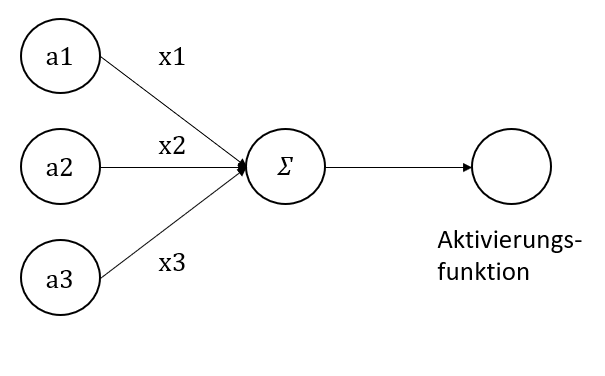
\includegraphics[width=0.6\textwidth]{images/h_nn.png}
	\caption{Darstellung eines Perzeptrons}
	\label{fig:h_nn}
\end{figure}

Um die Inputwerte so einfach wie möglich darzustellen, wird eine m x n-Matrix verwendet. Die folgende Matrix soll ein allgemeines Beispiel dafür zeigen. Jede Zeile dieser Matrix steht für einen Datensatz und der erste Wert steht für den Bias-Wert.

\[m = \begin{pmatrix}a_0 & a_1 & . & . & . & a_n \\  b_0 & b_1 & . & . & . & b_n \\ . \\ . \\ .\end{pmatrix}\]

\subsubsection{Die sigmoid-Aktivitätsfunktion}
\label{sec:inp}
Die sigmoid-Funktion ist die Aktivitätsfunktion der Layer, die im neuronale Netz aufgerufen wird. Da die Ergebnisse zwischen null und eins liegen, eignet sich diese Funktion für die Soll-Ergebnisse. \citep{Rey2011} Wichtig ist zu erwähnen, dass die Ergebnisse nicht den Wert null oder eins erreichen, sondern nur unter eins und über null liegen. Außerdem kann durch die möglichen Ergebnisse auch ein Intervall gewählt werden, bei dem die Klassifizierungen korrekt sind, auch wenn die Ergebnisse nicht exakt die gleichen sind. Damit ist der Raum der Ergebnismöglichkeiten größer und kann erweitert werden, sollten weitere Units im Output-Layer zu einem späteren Zeitpunkt dazu genommen werden.
\newline
\newline
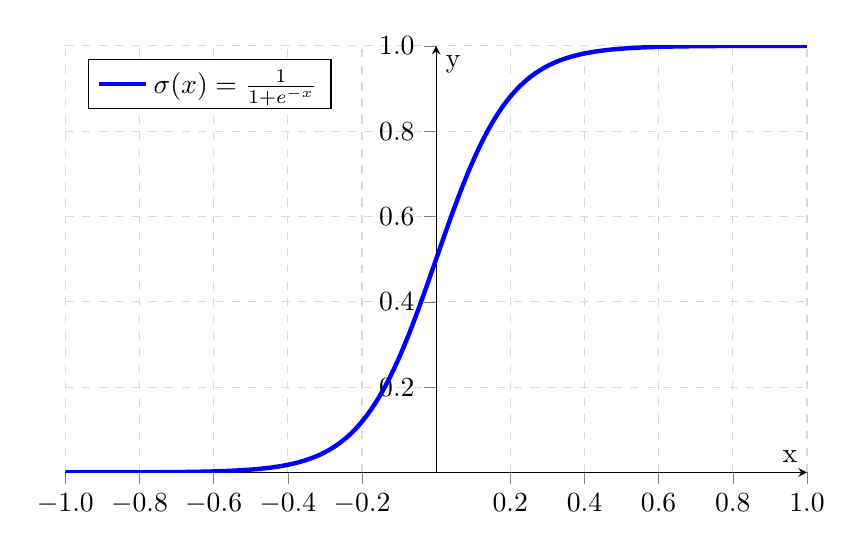
\begin{tikzpicture}
    \begin{axis}[
    	legend pos=north west,
        axis x line=middle,
        axis y line=middle,
        x tick label style={/pgf/number format/fixed,
                            /pgf/number format/fixed zerofill,
                            /pgf/number format/precision=1},
        y tick label style={/pgf/number format/fixed,
                            /pgf/number format/fixed zerofill,
                            /pgf/number format/precision=1},
        grid = major,
        width=11cm,
        height=7cm,
        grid style={dashed, gray!30},
        xmin=-1,     % start the diagram at this x-coordinate
        xmax= 1,    % end   the diagram at this x-coordinate
        ymin= 0,     % start the diagram at this y-coordinate
        ymax= 1,   % end   the diagram at this y-coordinate
        %axis background/.style={fill=white},
        xlabel=x,
        ylabel=y,
        tick align=outside,
        enlargelimits=false]
      % plot the stirling-formula
      \addplot[domain=-1:1, blue, ultra thick,samples=500] {1/(1+exp(-10*x))};
      \addlegendentry{$\sigma(x)=\frac{1}{1+e^{-x}}$}
    \end{axis}
\end{tikzpicture}

\subsubsection{Backpropagation}
Bei der Backpropagation läuft das neuronale Netz nochmal rückwärts ab, um die Gewichte so zu verändern, dass die Fehlerrate auf ein lokales oder globales Minimum reduziert wird. Man muss also im Netz rückwärts gehen und die Gewichte und Biases anpassen. Die Anpassung findet über das Gradientenabstiegsverfahren statt. \citep{Rey2011} beschreibt das Gradientenabstiegsverfahren. Wie schon in Kapitel \ref{sec:inp} genannt, verwendet das neuronale Netz die sigmoid-Funktion. Da hier aber die Backpropagation stattfindet, muss mit der partiellen Ableitung weiter gerechnet werden. Jede Gewichtung und jedes Bias der partiellen Ableitungen müssen im Gradienten Vektor gespeichert werden. Abschließen werden diese mit der Lernrate und der partiellen Ableitungen verrechnet. In Kapitel \ref{sec:ums_nn} wird die Umsetzung in der Programmiersprache Python dargestellt.
\newline

\[\displaystyle \frac{\partial \sigma(x)}{\partial x} = \sigma(x)(1-\sigma(x))\]

\newline
\newline
Die gezeigte Funktion ist die Ableitung der sigmoid-Funktion. Mit der Backpropagation wird die Cost-Funktion minimiert und es werden die Gewichte und der Bias-Wert in jedem Layer des neuronalen Netzes vom Output-Layer aus rückwärts angepasst.

\subsection{Ausgabe der Ergebnisse als Klassifizierung}
Das neuronale Netz des Prototypen arbeitet mit der Vorhersage, die Ergebnisse wie in Abbildung \ref{fig:nn_class} einzuteilen. Alle Punkte, die farblich eingeteilt sind, stehen für eine mögliche Klassifizierung. Dies bedeutet, dass ein Ergebnis aus dem neuronalen Netz einer dieser Klassen ist und die anderen Klassen einen Wert haben, welche nicht dem gewünschten Ergebnis entspricht. Also damit nicht die Klasse ist, in welches man das Ergebnis einteilt.

\begin{figure}[H]
	\centering
		%[natürliche Breite in Pixeln, natürliche Höhe in Pixeln, Abhängigkeit von der Textbreite]
		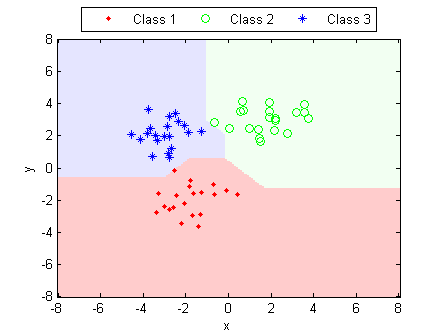
\includegraphics[width=0.75\textwidth]{images/nn_classifier.png}
	\caption{Beispiel einer Klassifizierung \citep{yuClass}}
	\label{fig:nn_class}
\end{figure}

In dieser Arbeit geht es darum, dass die Ergebnisse des neuronalen Netzes in Gruppen eingeteilt werden. Die visuelle Klassifizierung in der Abbildung \ref{fig:nn_class} ist nur ein Beispiel und entspricht nicht dem neuronalen Netz aus dieser Bachelorarbeit. Dennoch entsprechen diese drei Klasseneinteilungen, den Ergebnissen dem neuronalen Netz des Prototypen. Weiterhin ist relevant, dass diese Darstellung auch in Form eines Vektors erfolgen kann. Dies funktioniert aber nur bei einem Output-Layer mit mindestens zwei Units. Der folgende Vektor \(v\) zeigt eine weitere Möglichkeit, um die klassifizierten Ergebnisse darzustellen.
\newline

\[\displaystyle v = \begin{bmatrix}y_1 \\ y_2 \\ . \\ . \\ . \\ y_n\end{bmatrix}\]

\subsection{Die Trainingsphase und Testphase mit Einlesen von Testdaten}
\label{subsec:eval}
Bei einem neuronalen Netz gibt es zwei Phasen - die Trainings- und die Testphase. Diese werden durch ein Dataset repräsentiert, welches Trainingsdaten und Testdaten beinhaltet. Während der Trainingsphase werden ein Teil dieses Datasets in das neuronale Netz als Inputwerte eingegeben und über Supervised Learning trainiert. Das Supervised Learning beschreibt eine Lernmethode, bei der die Trainingsdaten mit den Soll-Ergebnissen trainieren. Es wird schon beim Training das richtige Ergebnis mitgeteilt. Da die Gewichte, deren Aufgabe in Kapitel \ref{sub:fee_back} näher erläutert wird, zu Beginn noch willkürlich gewählt sind, werden diese in der Trainingsphase angepasst.   
\newline
Sind die Gewichte angepasst, erfolgt die Testphase. In der Testphase wird getestet, wie gut das neuronale Netz voraussagen kann, was das richtige Ergebnis ist. Es wird nicht mehr das Ergebnis wie beim Training vorgesagt. Ziel dieses Vorgangs ist danach weitere Echtzeitwerte in das neuronale Netz einzugeben und  durch das Trainig und den Tests die richtige Klassifizierung vorherzusagen.
\newline
Das neuronale Netz muss so programmiert werden, dass es mit dem Dataset trainiert und getestet werden kann. Also klappt es nicht, wenn es z.B. eine Bildklassifizierung vorhersagen müsste, welches Vorhersagen beim Boston-Housing Dataset durchführt.
 
\section{MQTT zur Datenübertragung}
\label{sec:mqtt}
MQTT ist ein M2M-Protokoll, welches mit der Publish-Subscribe-Methode arbeitet. Mikrocontroller und Sensoren publishen dabei ihre Daten an den MQTT-Broker. Der Broker speichert diese Daten zwischen, bis Subscriber diese Nachrichten anfordern. Jeder Subscriber bekommt diese Nachrichten gleichzeitig je nach Quality of Service Stufe zugestellt. Diese Clients können ihre Daten wiederum auch publishen und wieder an neue Geräte die als Subscriber markiert sind, versenden. Als Clients sind intelligente Geräte gemeint, wie Mikrocontroller oder PCs. Ein Client ist Subscriber, Publisher oder beides zusammen. Die Anzahl der Clients, die aktiv als Subscriber oder Publisher dienen, ist nicht relevant. Wichtig ist dabei nur, dass der Broker funktioniert und verfügbar für die Clients ist.\citep{soni2017survey} Damit eignet sich dieses Protokoll für den IoT-Bereich besonders gut.
\newline
Wie schon gesagt, werden die Narichten je nach QoS Stufe versendet. Es gibt insgesamt drei Stufen des QoS. Diese werden in der Tabelle \ref{tab:tableqos} dargestellt. Die Stufen dienen zur Sicherung der Nachrichtenübermittlung, auch wenn das Netz dabei gestört wird. So sollen die Nachrichten trotzdem weiterhin vermittelt werden.

\begin{table}[H]
	\centering
	\caption[Tabellarische Darstellung der QoS Level]{Tabellarische Darstellung der QoS Level \citep{soni2017survey}}
		\vspace{1.0em}	
	\begin{tabular}{| l | l | p{5cm}|}
		\hline
		\rowcolor[gray]{0.9}\textbf{Stufen} & \textbf{Häufigkeit} & \textbf{Beschreibung} \\
		\hline
		\hline
		0 & höchstens eine Nachricht & Es wird maximal eine Nachricht versendet, ohne eine Garantie, dass diese auch ankommt \\
		\hline
		1 & mindestens eine Nachricht & Es ist möglich, dass eine Nachricht mehr als einmal versendet wird \\
		\hline
		2 & genau eine Nachricht & Eine Nachricht wird mit einem Four-Way Handshake versendet \\
		\hline
	\end{tabular}
	\label{tab:tableqos}
\end{table}
\newline
Für die Kommunikation ist ein TCP-Stack und das MQTT-Protokoll vorausgesetzt. Zusätzlich ist eine Verbindung zum MQTT-Broker erforderlich bei dem der Typ des Netzes aber unwichtig ist. Außerdem ist zu erwähnen, dass es nicht relevant ist, dass sowohl Publisher als auch Subscriber gleichzeitig aktiv sein müssen. Der Broker kann die Nachrichten auch dann noch übermitteln, obwohl der Publisher nicht mehr aktiv ist.
\newline
Damit Nachrichten versendet werden, gibt es die sogennanten Topics. Bei diesen Topics ist es nicht wichtig, über welche Struktur die Nachricht aufgebaut ist. \citep{Trojan2017} MQTT ist mit dieser Methode ein Protokoll, welches passend für diesen Prototypen ist, da es für das Senden von Sensordaten in einem Wireless Network ausgelegt ist. 

\section{Sensoren für die Interaktionen auf dem Sofa}
Die Sensoren sind ein Hauptbestandteil des Prototyps. Diese sind mit Mikrocontrollern verbunden und ein Raspberry Pi sorgt für die Kommunikation zwischen den Geräten und den Mikrocontrollern. Neben der Erläuterung der genutzten Sensoren in dem aktuellen Prototyp wird hier auch zusätzlich der Mikrocontroller und Raspberry Pi beschrieben.

\subsection{Erläuterung des Raspberry Pi 3 und des ESP32}
Der Raspberry Pi 3 ist ein Einplatinencomputer, auf dem das Betriebssystem Raspbian installiert ist. Das Betriebssystem basiert auf Linux Debian und läuft in der aktuellen Version 10 - Buster. Neben den Möglichkeiten den Raspberry Pi für einfachere Anwendungen zu Verwenden, ist es auch möglich verschiedene Sensoren an dessen GPIO-Pins anzuschließen. Der Raspberry Pi 3 hat einen einen internen WiFi-Chip und kann damit in einem WLAN-Netzwerk eingebunden werden. Dies wird benötigt, da der Prototyp in einem lokalen Netzwerk ausgeführt wird.
\newline
Der ESP32 hingegen ist ein Mikrocontroller, welcher als Nachfolger vom ESP8266 weitere GPIO Pins besitzt, um mehr als einen Analogen Sensor anschließen zu können. Dies ist wichtig, da für den Prototypen mehrere Analog-Sensoren angeschlossen werden müssen. Ein ESP32 hat ein Live Betriebssystem und kann nur ein Programm ausführen, welches vorher auf den ESP geladen werden muss. 

\begin{figure}[H]
	\centering
		%[natürliche Breite in Pixeln, natürliche Höhe in Pixeln, Abhängigkeit von der Textbreite]
		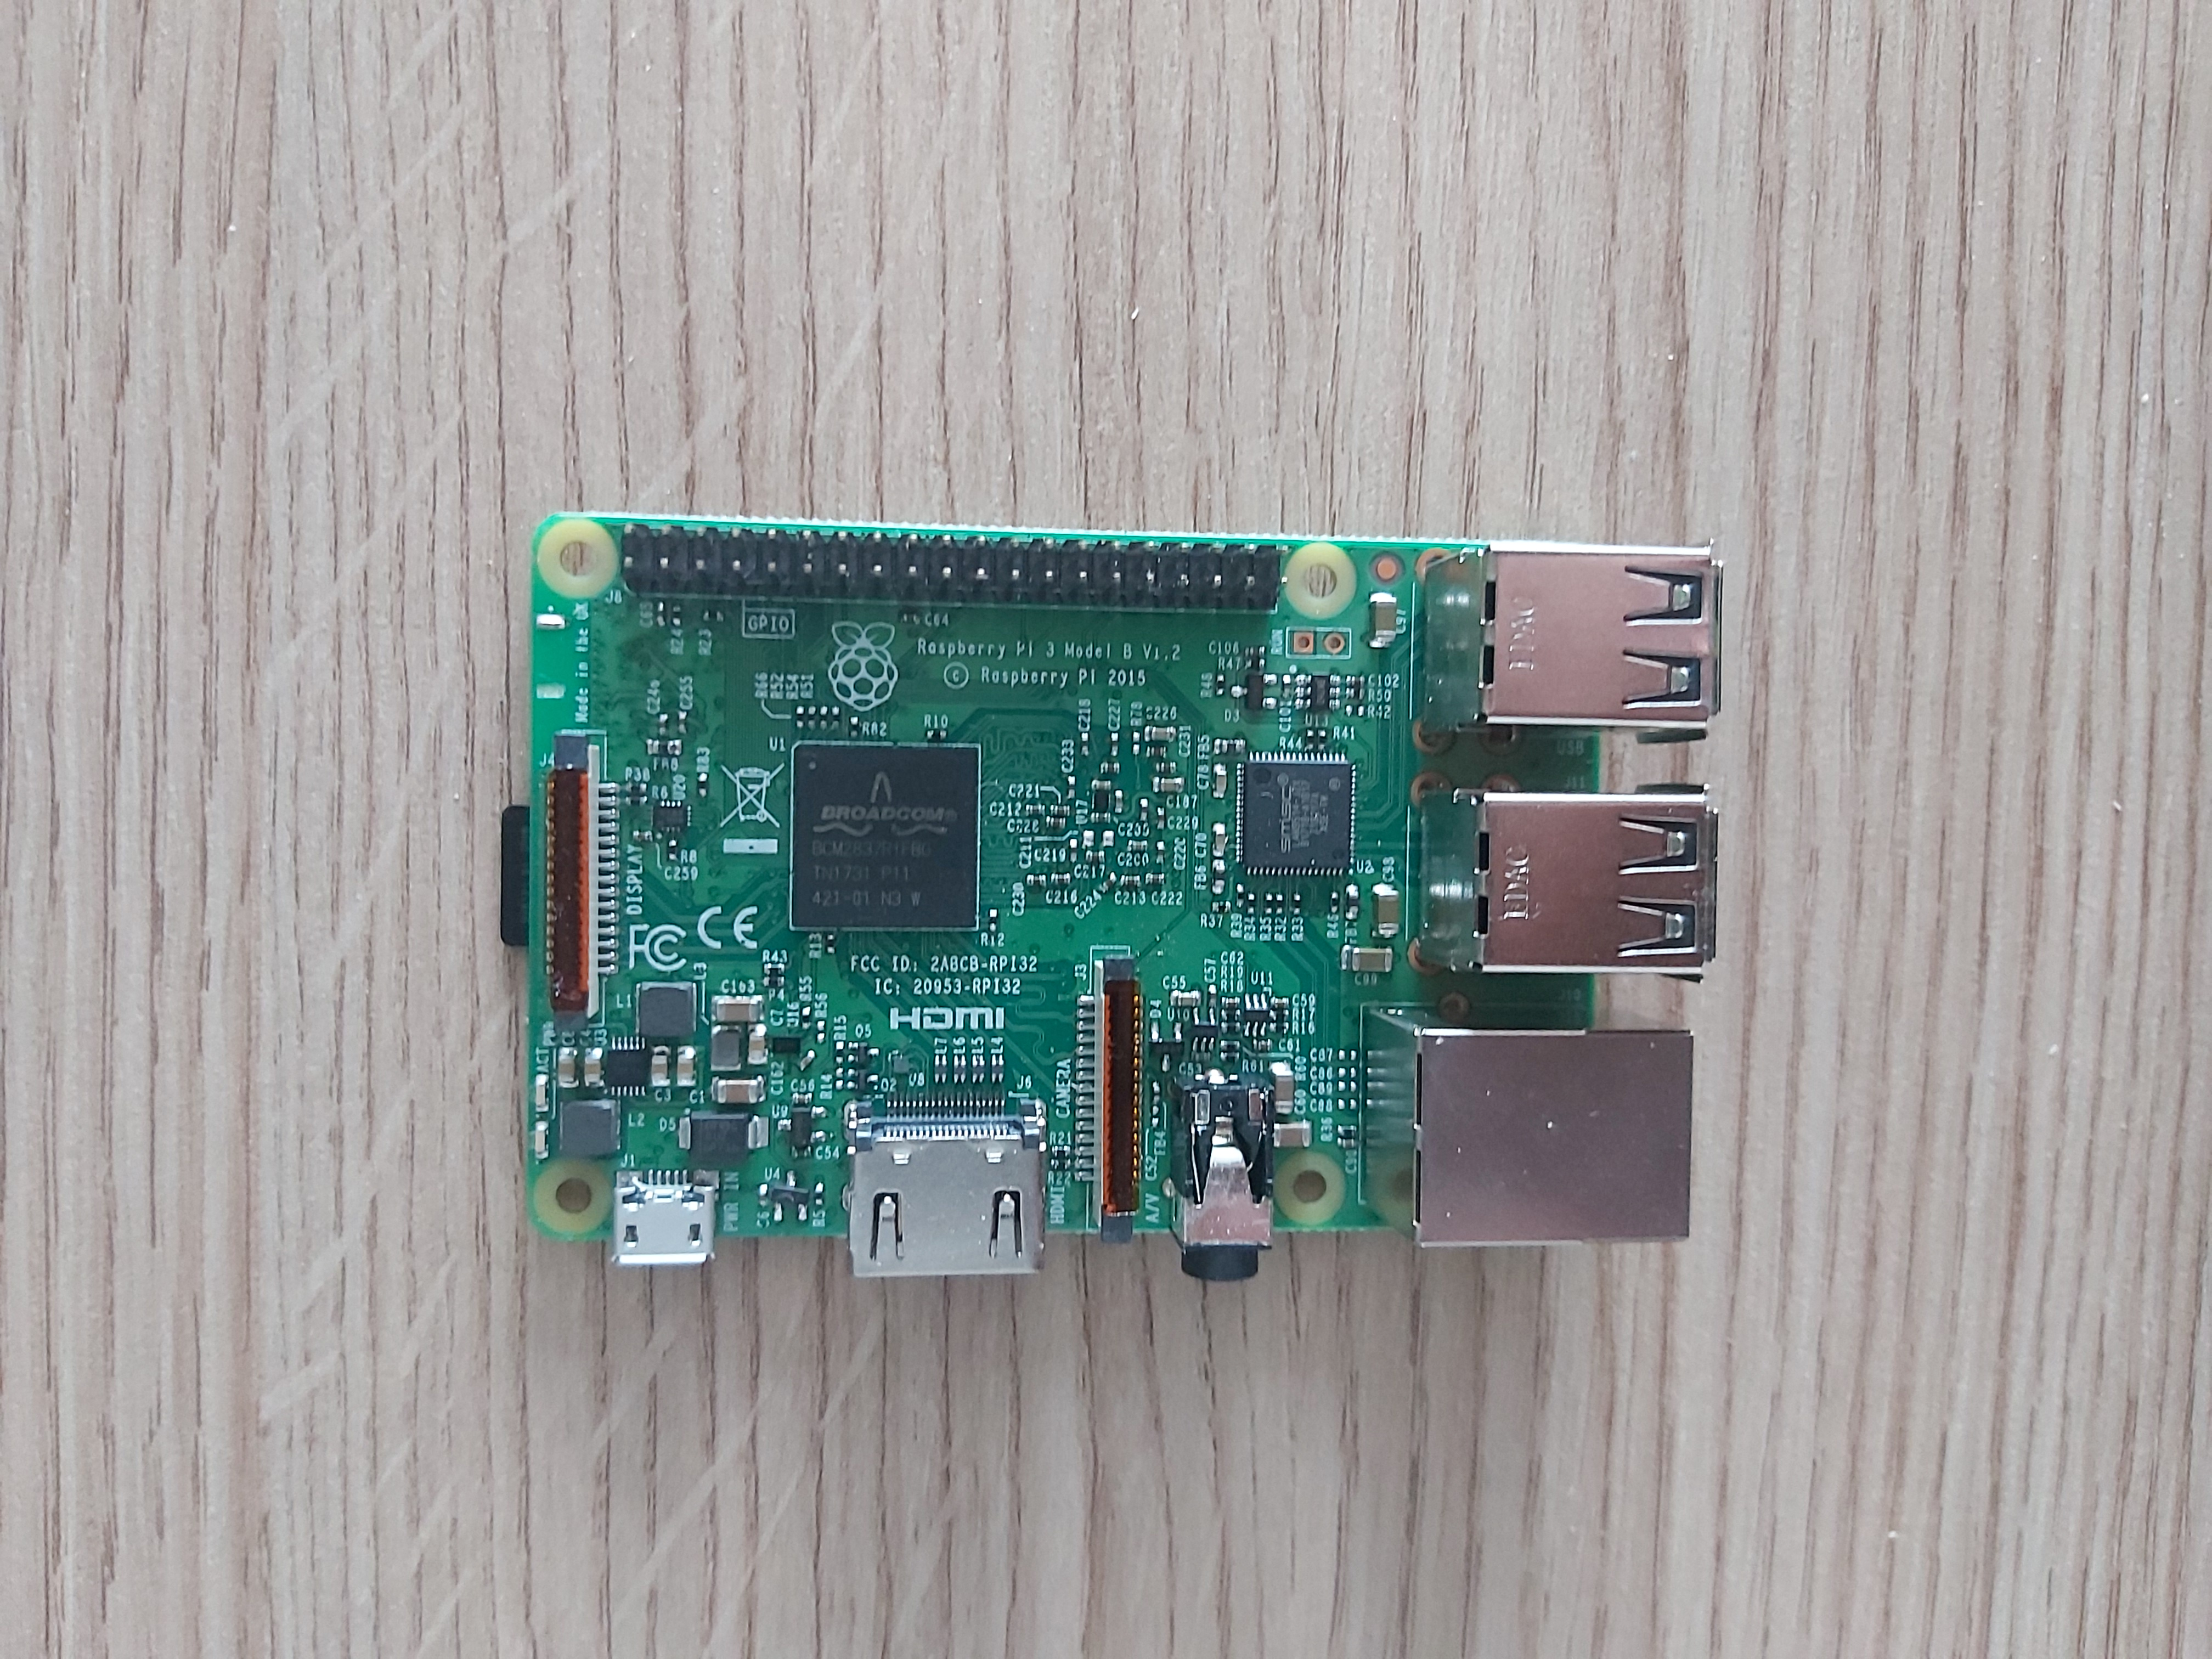
\includegraphics[width=0.49\textwidth]{images/r_pi.jpg}
		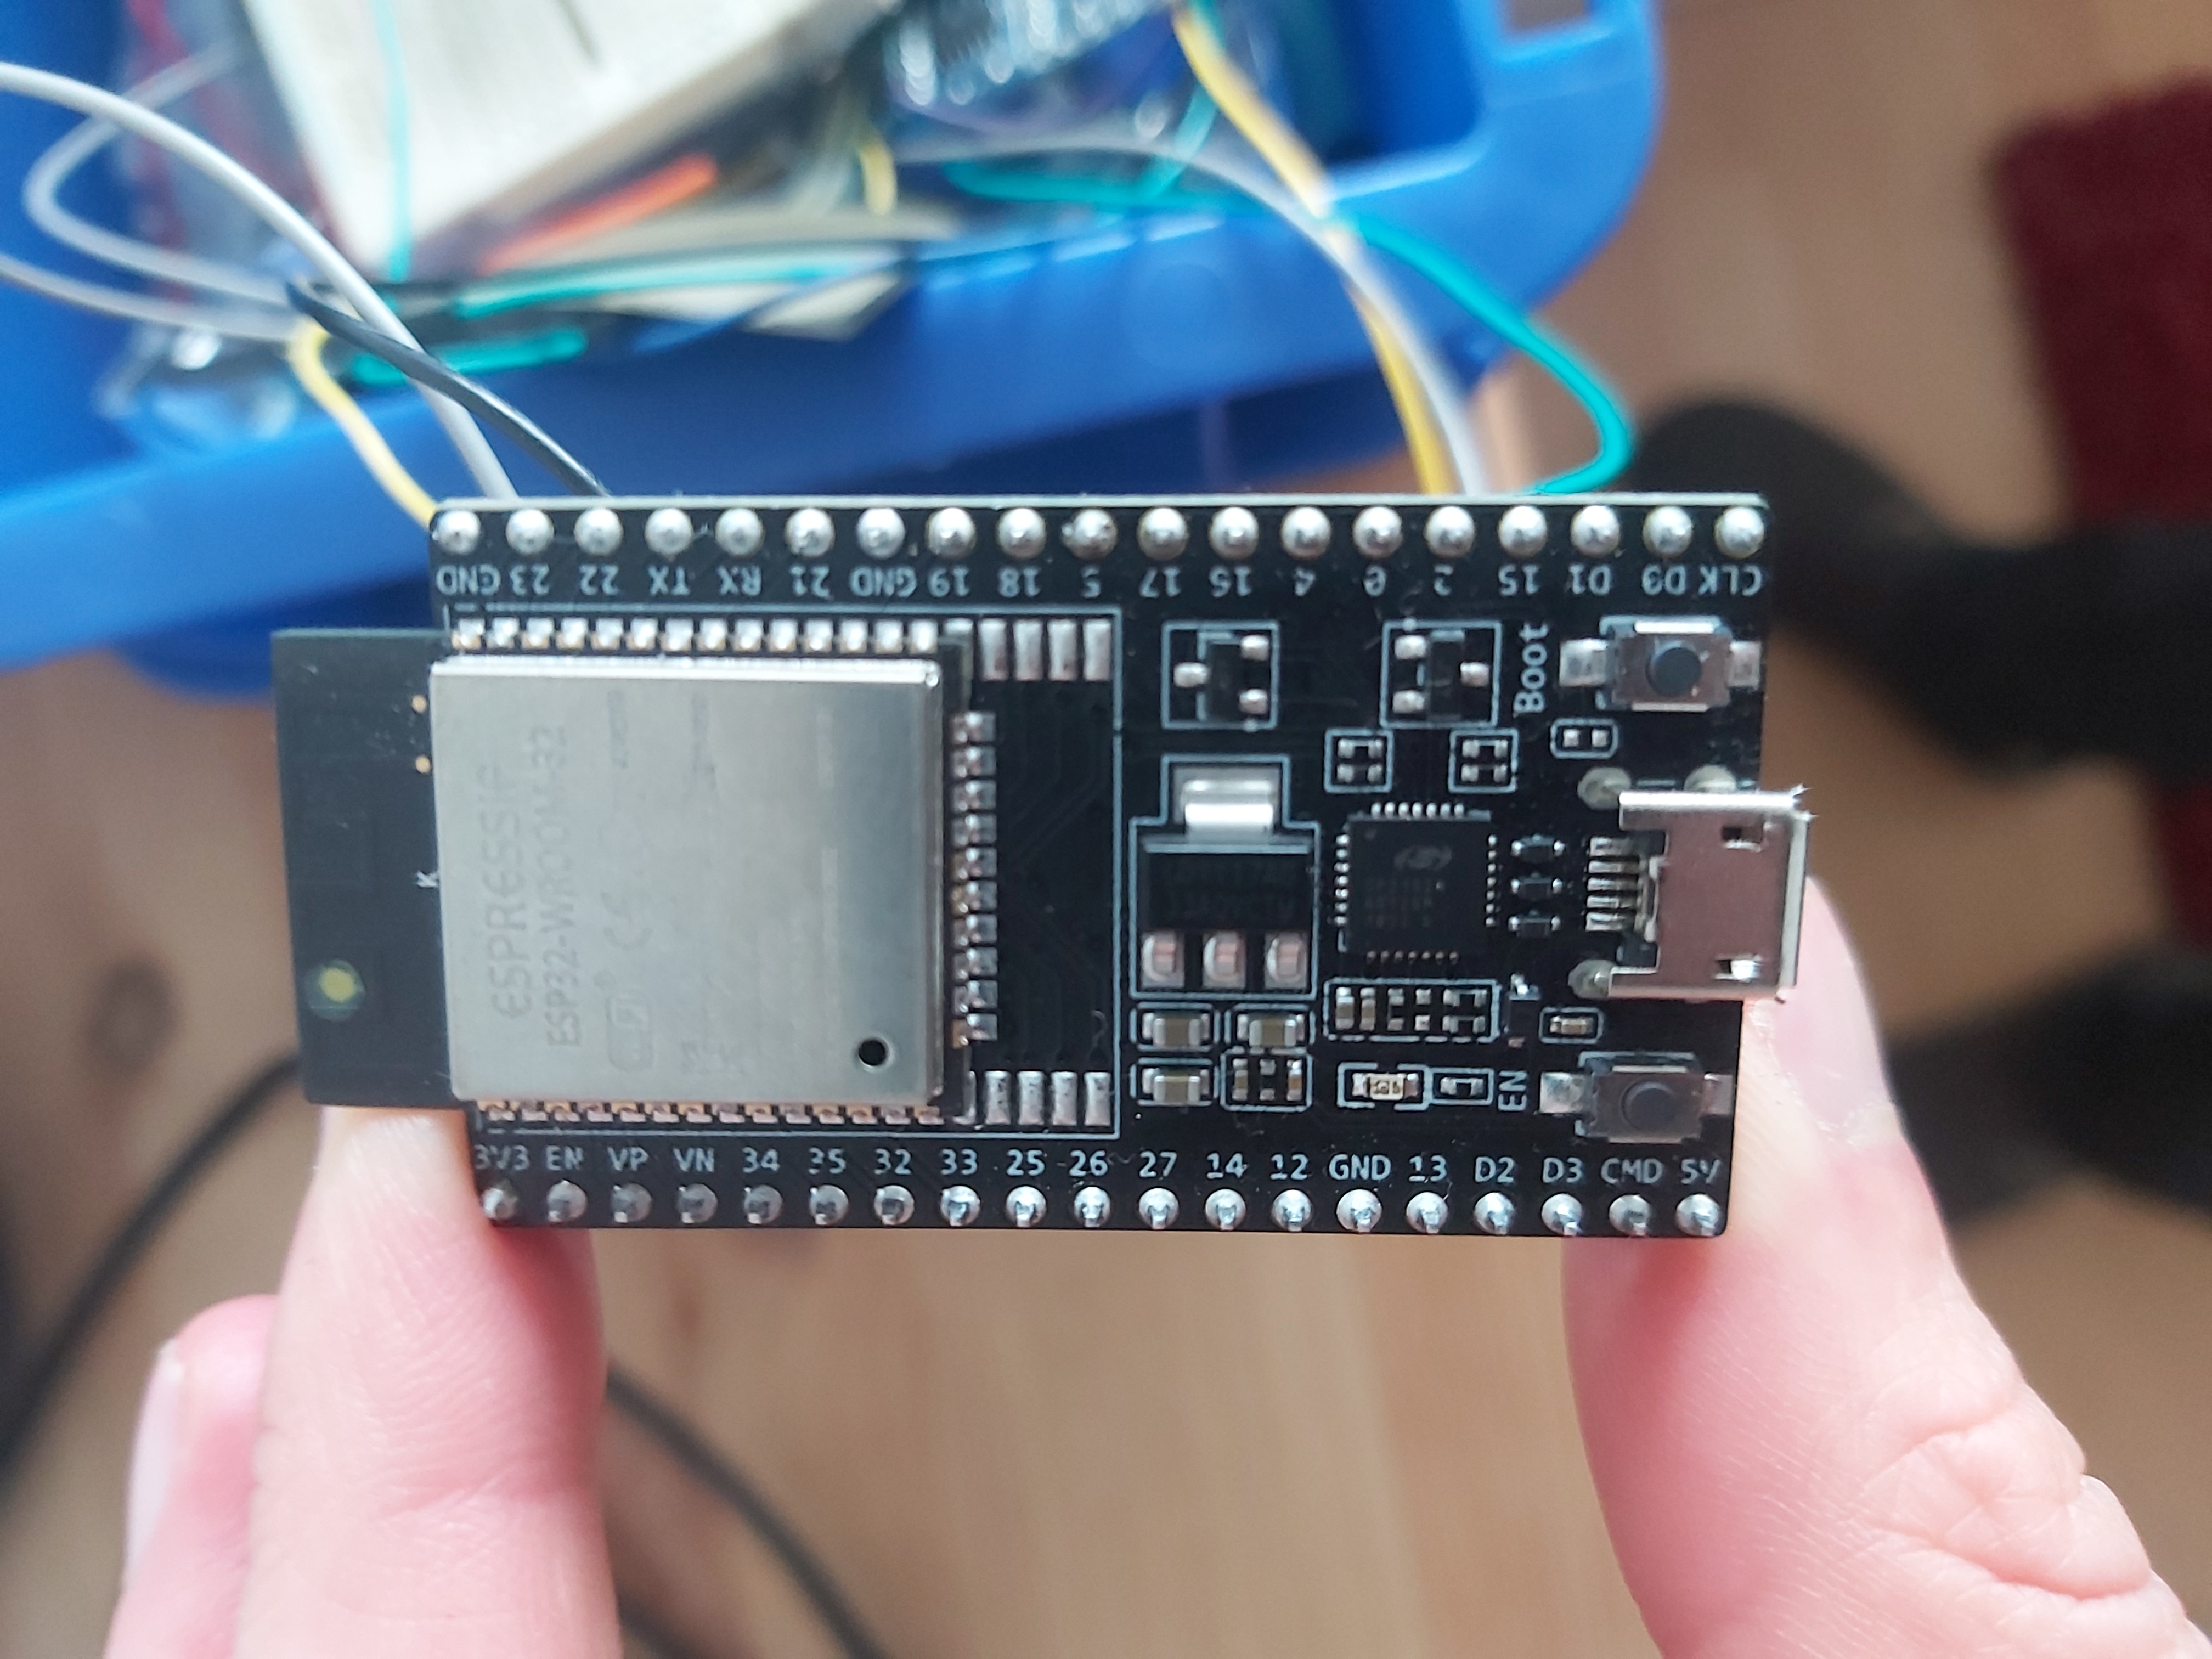
\includegraphics[width=0.49\textwidth]{images/esp_32.jpg}
	\caption{Die linke Abbildung zeigt den Raspberry Pi und die Rechte den ESP32}
	\label{fig:hardware}
\end{figure}

\subsection{Sensoren, die für den Prototypen verwendet werden}
Für den aktuellen Prototypen werden Ultrasonic-Sensoren und Force Sensitive Resistors verwendet. 
Diese reichen aus, um Sitz- und Liegepositionen der Nutzer zu erkennen. Dennoch zeigt Kapitel \ref{sec:er_in} die Vor- und Nachteile der Sensoren in der Realanwendung. \citep{de2018obstacle} beschreibt die Funktionen des Ultrasonic-Sensors in der fremden wissenschaftlichen Arbeit. Wichtig ist dabei herauszulesen, dass der Sensor Distanzen zwischen 1 cm und 4 Meter messen kann. So ist dieser Sensor eine gute Möglichkeit, um auch Personen zu erkennen die sich anlehnen. Das Problem ist allerdings, dass beim Verwenden dieses Sensors im Prototypen dieser im Sofa verbaut sein muss. Dadurch können sich Personen so anlehnen, ohne den Sensor physisch zu treffen. Zudem ist der Radius, in dem die Wellen gesendet werden, zu gering, da die Sofalehnen mehr Platz haben als der Sensor messen kann.
\newline
Neben dem Ultrasonic-Sensor misst der FSR-Sensor anhand des elektrischen Widerstands den Druck, welcher zwischen 100 Gramm und 10 kg beträgt. Bei allen Gewichten über 10 kg zeigt der Sensor immer den höchsten Wert. \citep{florez2010calibration} Der Sensor ist aus zwei Polymerschichten gebaut. Eine leitende Oberfläche und die zweite, welche an die erste Schicht mit Elektroden gebunden ist. \citep{hollinger2006evaluation} Diese Sensoren werden verwendet, um zu erkennen, wann die Personen Druck auf sie ausüben indem sie ihn mit ihrem Gewicht auslösen. Als FSR-Sensoren werden die interlink Sensoren eingesetzt. Abbildung \ref{fig:sensors} zeigt die Sensoren, welche am ESP32 verbaut sind. Die beiden gezeigten FSR-Sensoren sind unterschiedlich groß, geben aber die gleichen Werte aus.

\begin{figure}[H]
	\centering
		%[natürliche Breite in Pixeln, natürliche Höhe in Pixeln, Abhängigkeit von der Textbreite]
		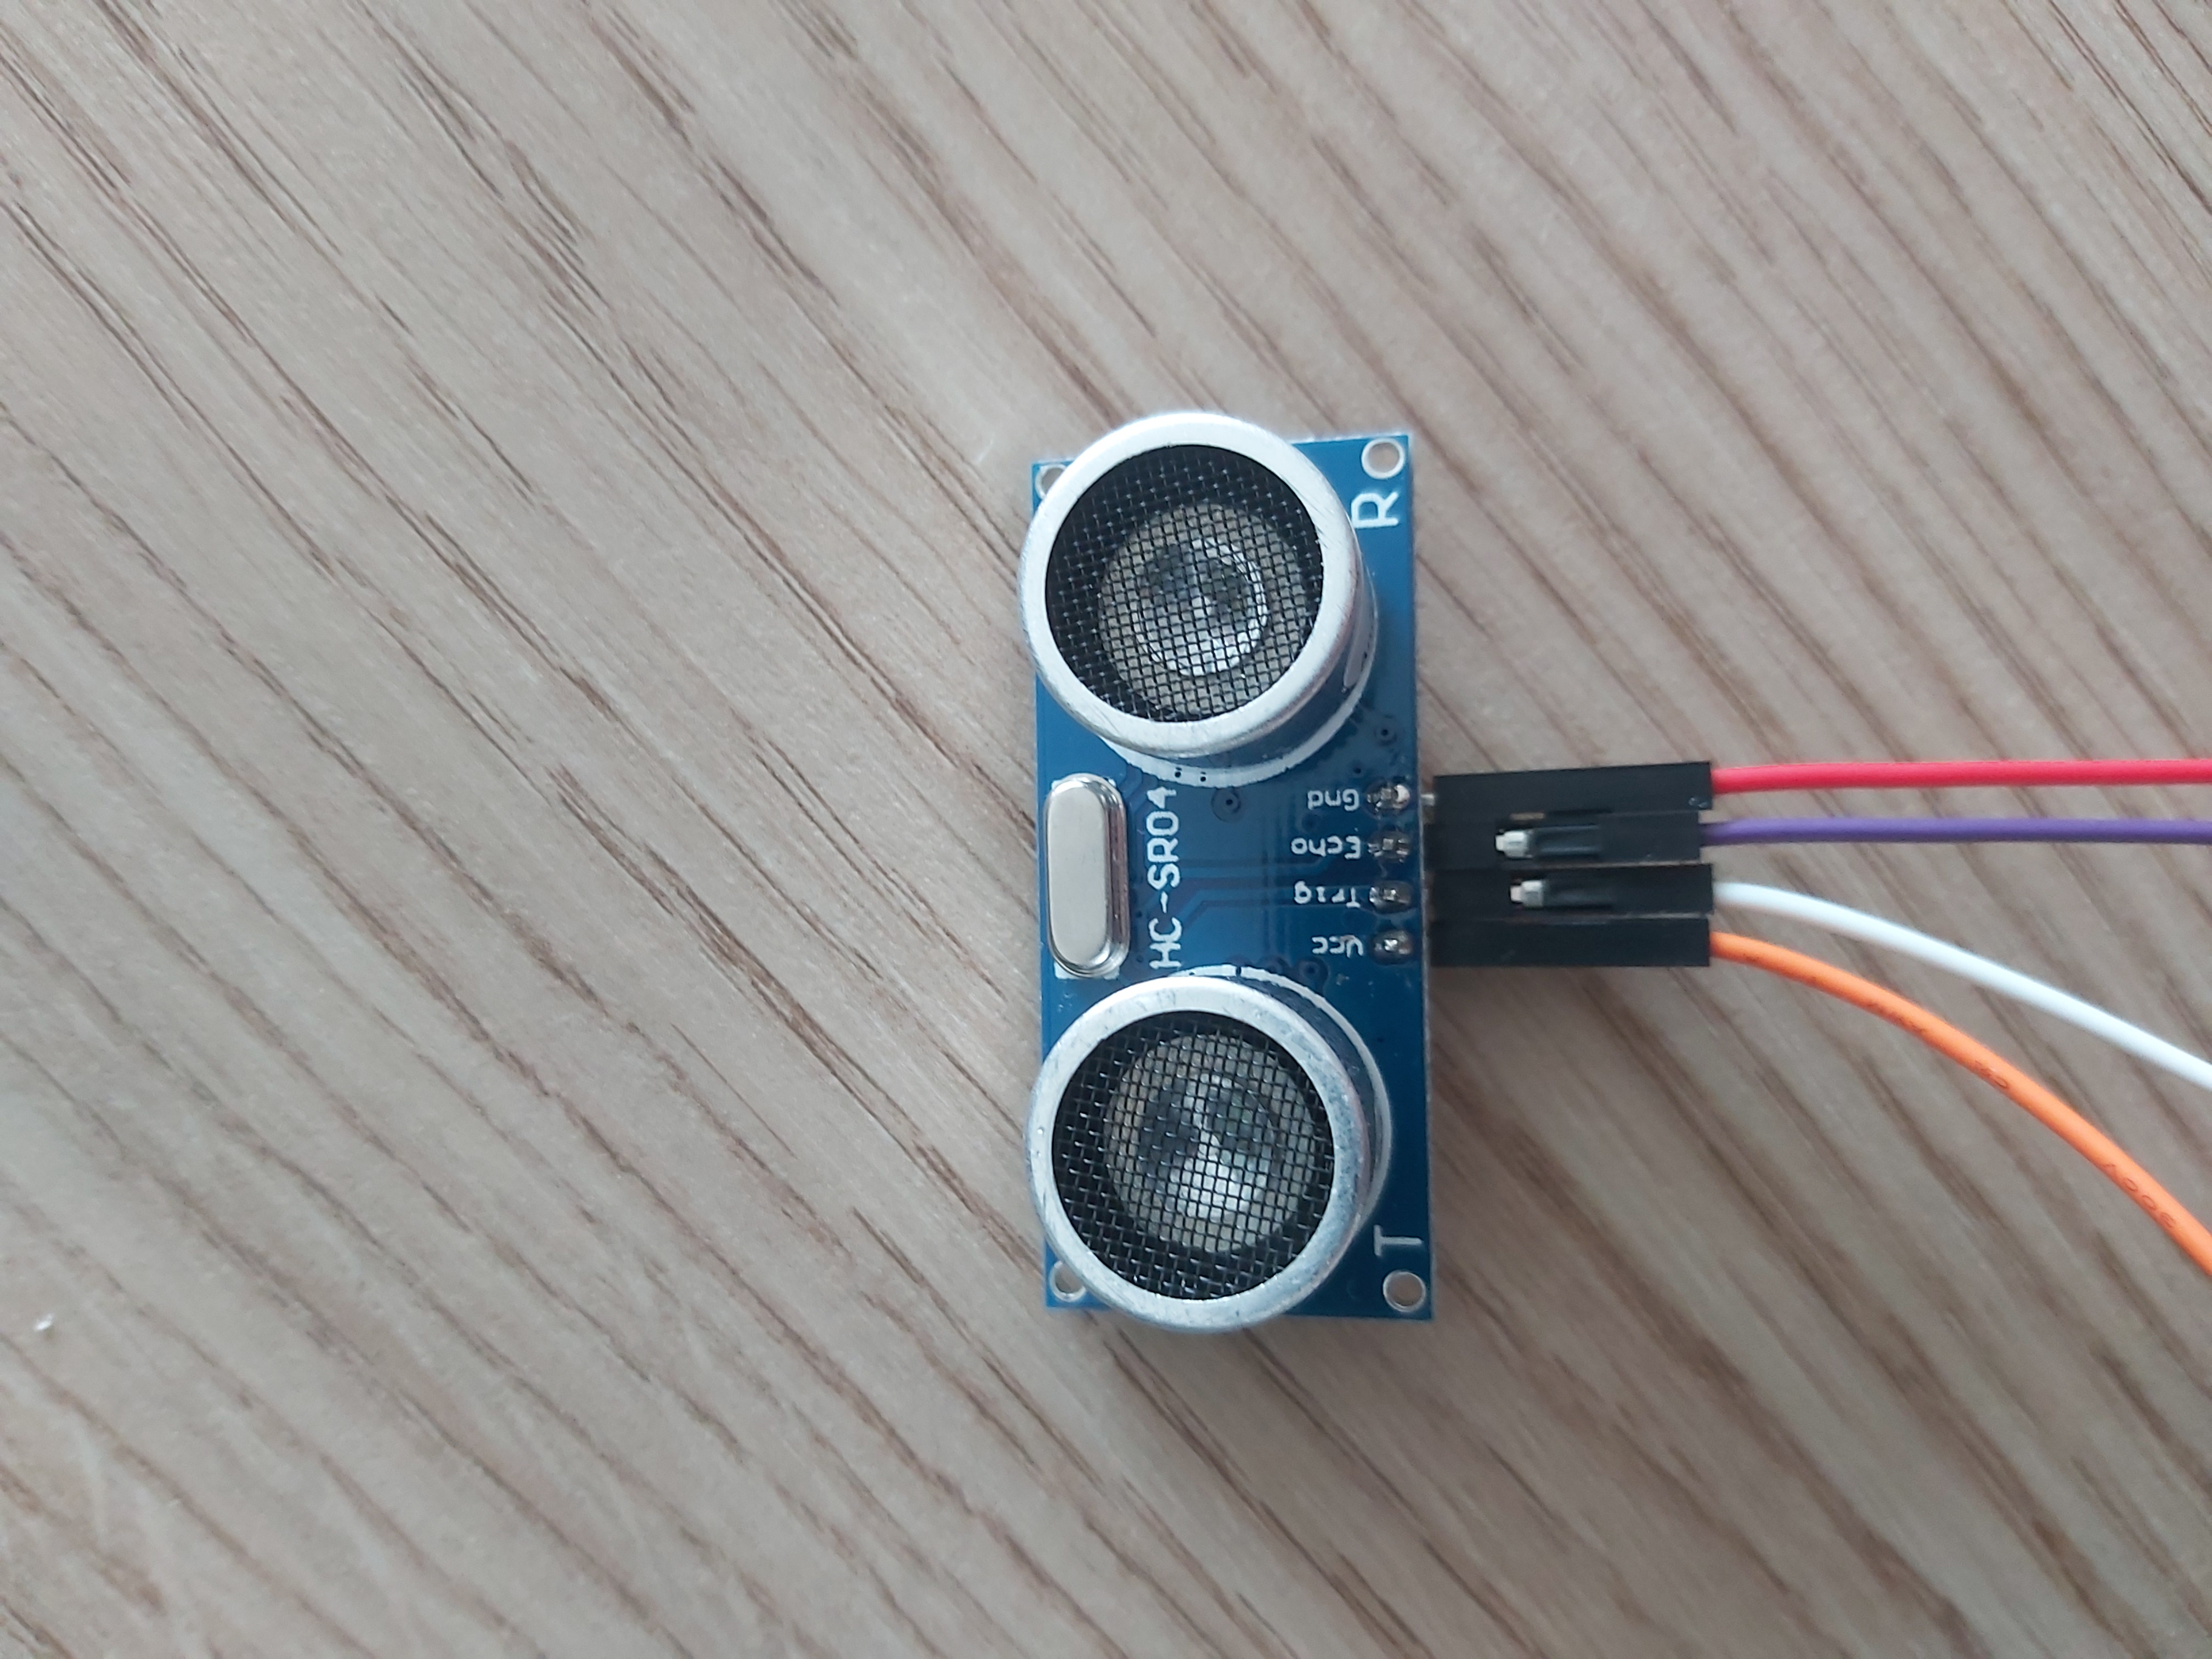
\includegraphics[width=0.32\textwidth]{images/ult_son.jpg}
		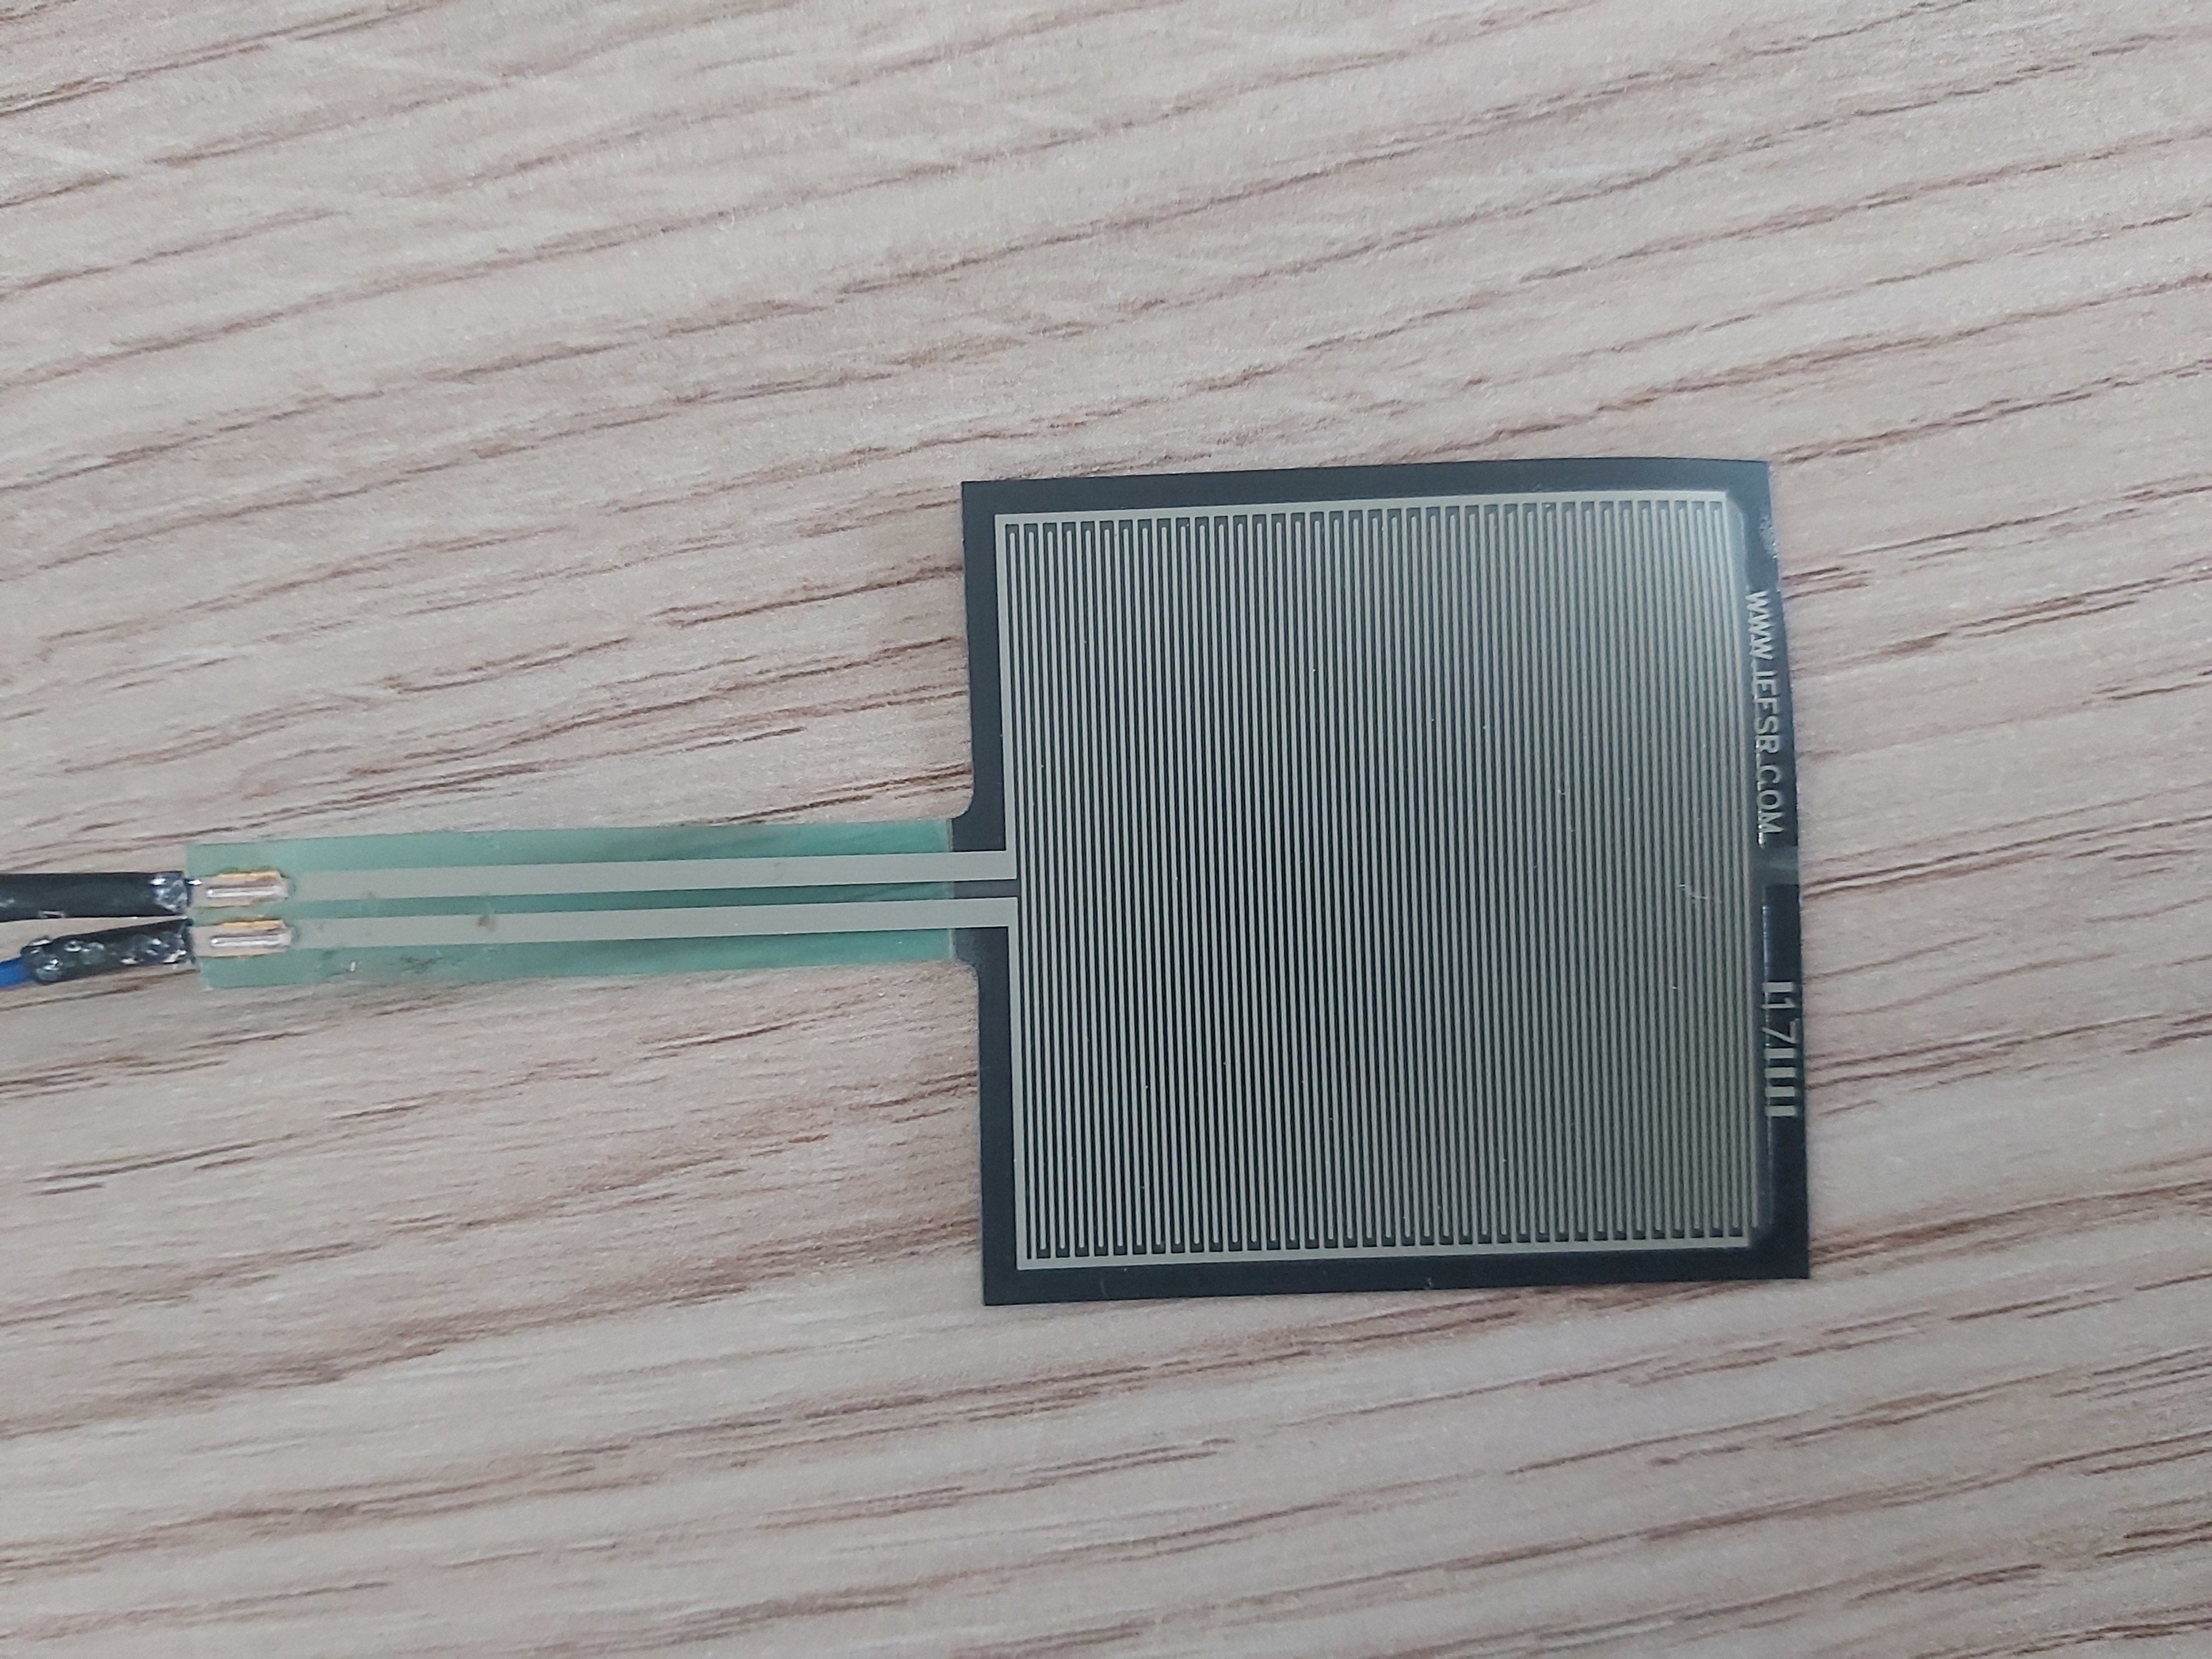
\includegraphics[width=0.32\textwidth]{images/fsr_gross.jpg}
		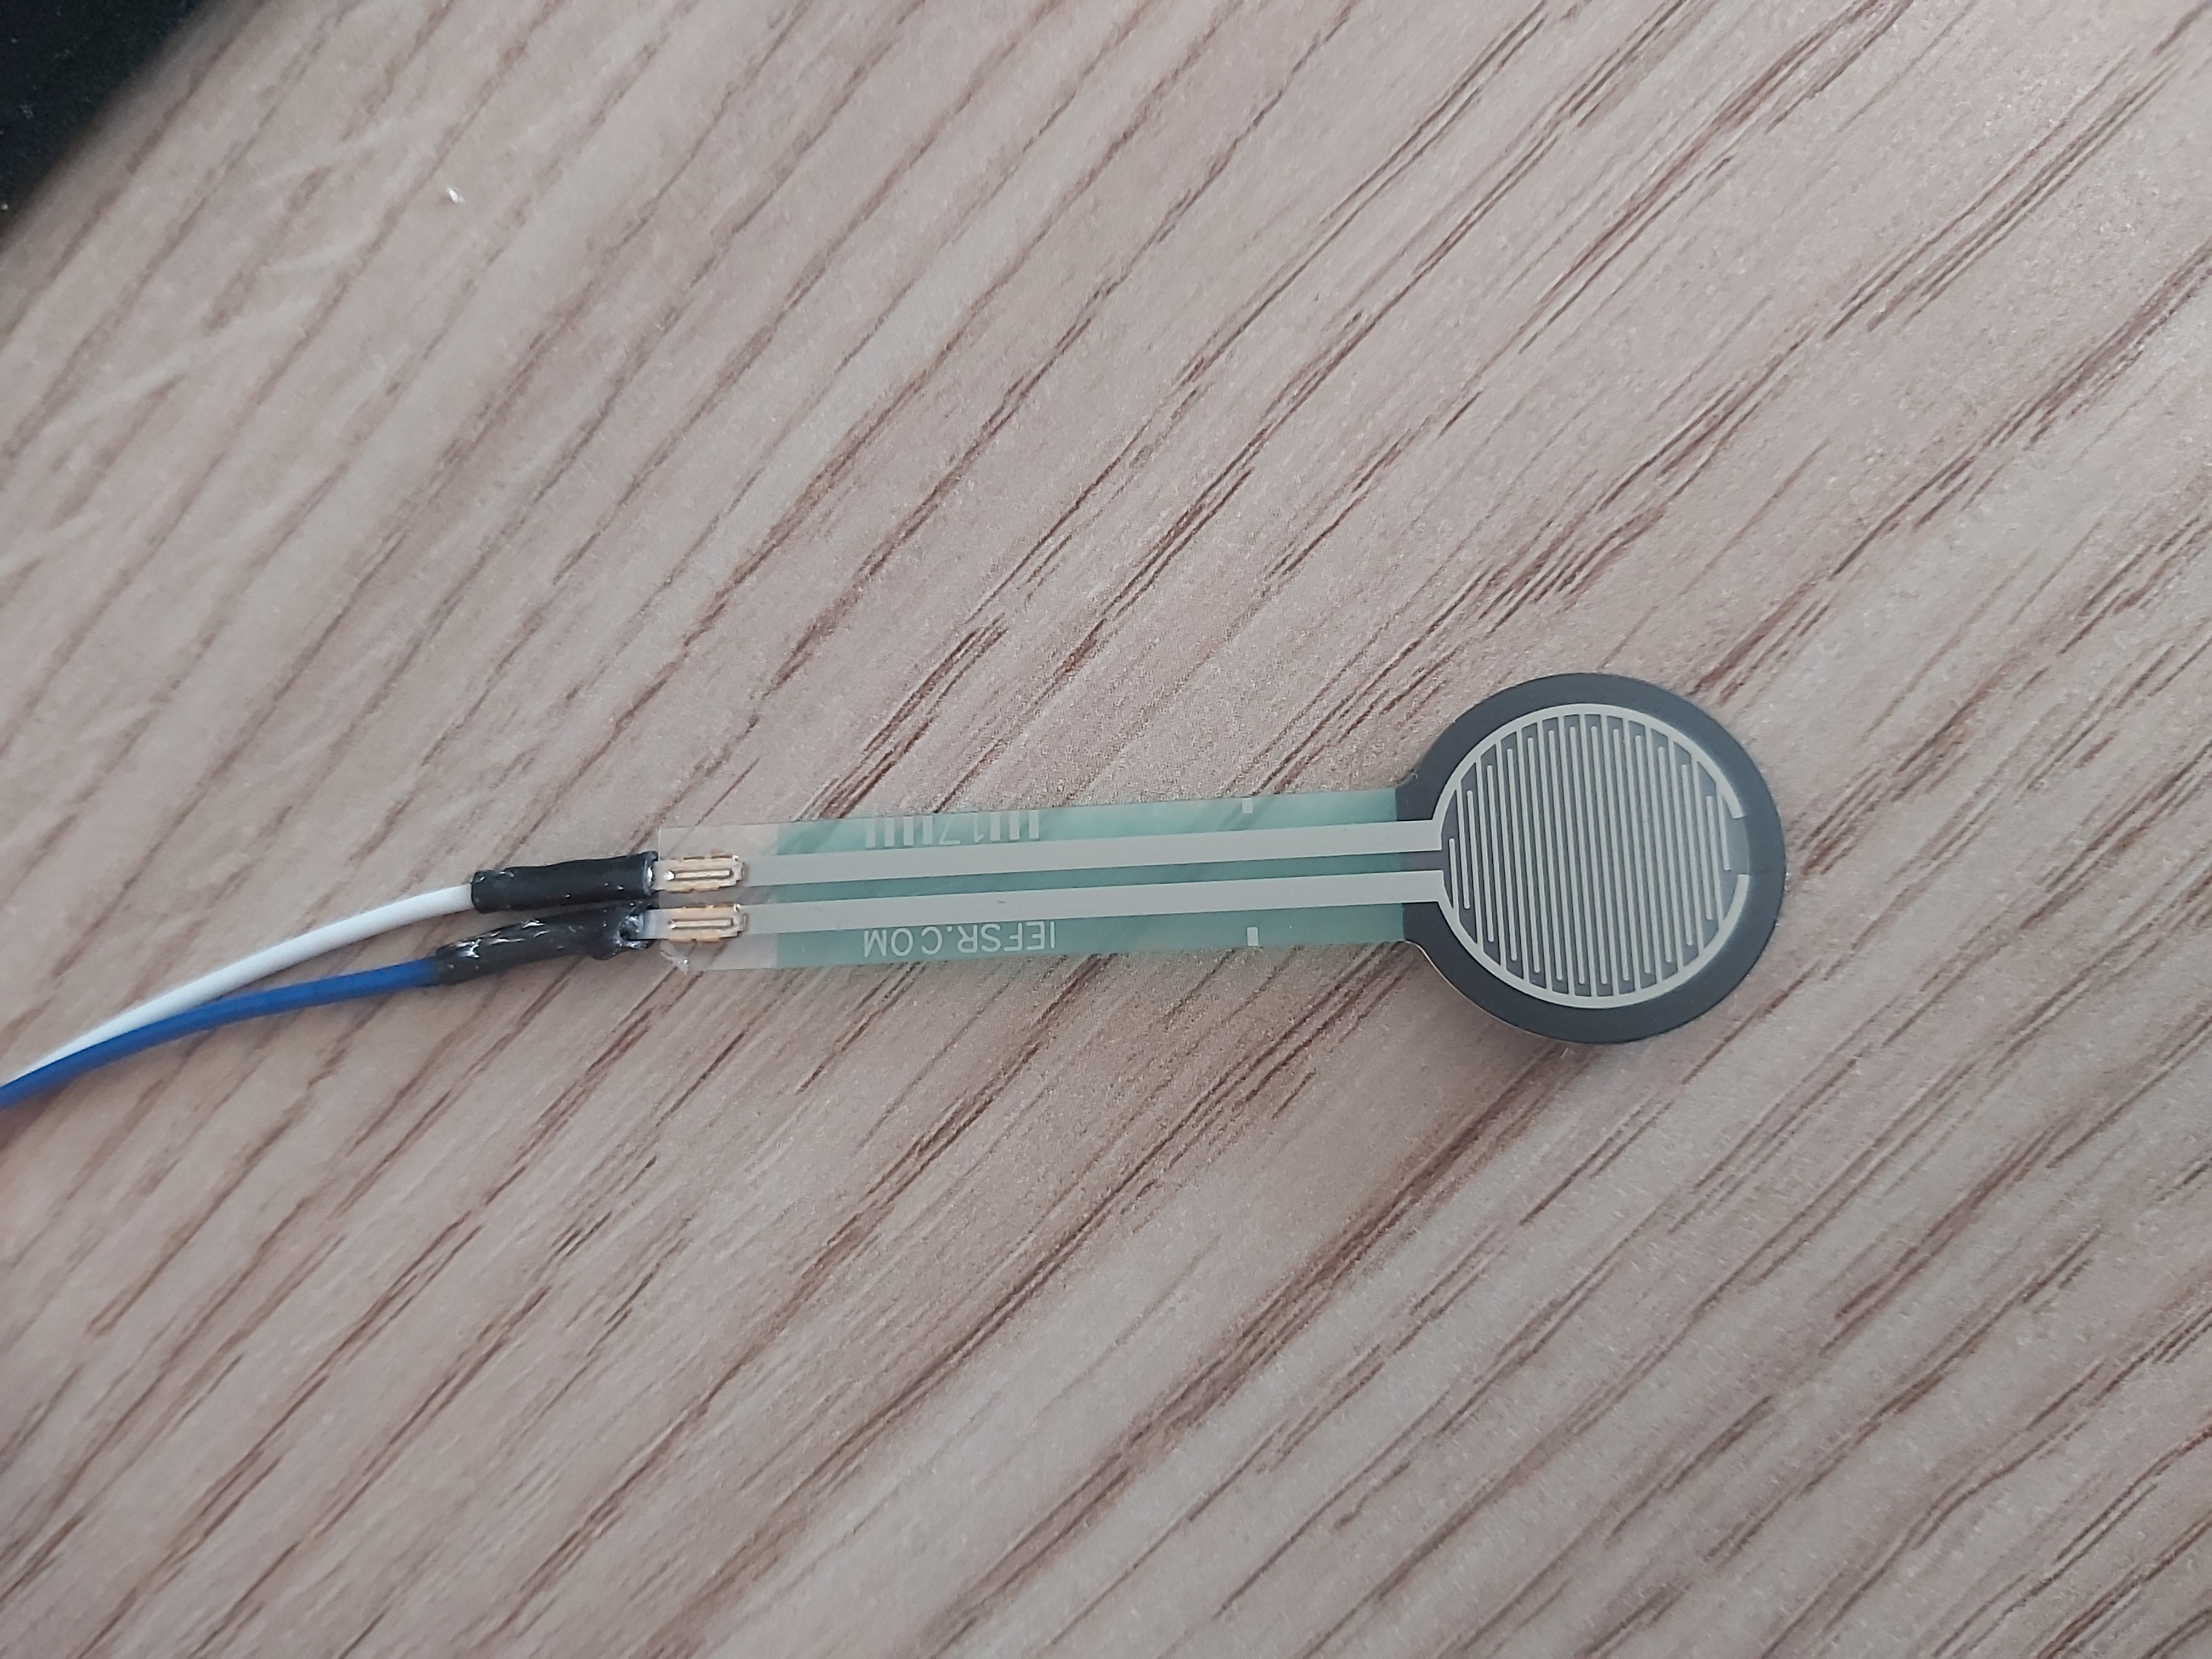
\includegraphics[width=0.32\textwidth]{images/fsr_klein.jpg}
	\caption{Links ist der Ultrasonic-Sensor, in der Mitte der Große und rechts der kleine FSR}
	\label{fig:sensors}
\end{figure}

\section{Prototyp aus dem Praxisprojekt}
Als letzten Punkt geht der Autor nochmal auf den Prototyp im Praxisprojekt ein. Der Prototyp, welcher die Interaktionen als Regelsystem mit sieben Regeln verwaltet, ist ein Projekt, welches im Rahmen des Praxisprojekts entwickelt wurde. Ein ESP32 misst die Sensordaten von zwei FSR-Sensoren und einem Ultrasonic-Sensor. Jeder Sensor wird als MQTT-Client deklariert und sendet Daten in Form von Codes, je nachdem mit welchen Sensoren der Nutzer interagiert. Zusätzlich messen zwei ESP8266 die Daten von jeweils einem Flex-Sensor, welche den Widerstand durch ihre Biegung messen. \citep{saggio2015resistive} Dies erweist sich aber als Nachteil, da die Biegung erst ab 45 Grad gemessen wird. Das kommt beim Test als Ergebnis heraus, durch Biegungen ohne auf ihm zu liegen und beim Testen des kompletten Prototypen. 
\newline
Ein Raspberry Pi 2 führt einen MQTT-Broker Service aus. Er kann Daten von den ESP-Sensoren empfangen, die über die Publish-Methode die Codes versenden. Auf dem Raspberry Pi 2 läuft zusätzlich ein Python-Programm, welches die Codes als Subscriber empfängt und im Regelsystem verwaltet. Die Regeln werden als Codes neu an den MQTT Broker gepublished. Daraufhin können die Codes dann von jedem beliebigen Subscriber empfangen werden. \citep{Schroeder2019} 
\newline
Was bei der Nutzung des Regelsystems aber nicht beachtet wurde, sind die Ausreißer der FSR-Sensorwerte. Mit dem Regelsystem zielt man darauf ab, dass die FSR-Sensoren immer wenn sie Nichtbenutzt werden, den Wert 0 haben und wenn sie besetzt sind, den Wert 1024. Während des Tests sind diese Ausreißer immer wieder aufgefallen. Da wird der Fall ausgelöst, dass der FSR-Sensor eine Interaktion erkennt, obwohl keine stattfindet.
